% File tacl2018v2.tex
% Sep 20, 2018

% The English content of this file was modified from various *ACL instructions
% by Lillian Lee and Kristina Toutanova
%
% LaTeXery is mostly all adapted from acl2018.sty.

\documentclass[11pt,a4paper]{article}

%% Package options:
%% Short version: "hyperref" and "submission" are the defaults.
%% More verbose version:
%% Most compact command to produce a submission version with hyperref enabled
%%    \usepackage[]{tacl2018v2}
%% Most compact command to produce a "camera-ready" version
%%    \usepackage[acceptedWithA]{tacl2018v2}
%% Most compact command to produce a double-spaced copy-editor's version
%%    \usepackage[acceptedWithA,copyedit]{tacl2018v2}
%
%% If you need to disable hyperref in any of the above settings (see Section
%% "LaTeX files") in the TACL instructions), add ",nohyperref" in the square
%% brackets. (The comma is a delimiter in case there are multiple options specified.)

\usepackage{times,latexsym}
\usepackage{url}
\usepackage{amsthm}
\usepackage{amsmath}
\usepackage[utf8]{inputenc}
\usepackage{todonotes}
\usepackage[english]{babel}
\usepackage[style=american]{csquotes}
\usepackage[]{tacl2018v2}
\usepackage{graphicx}


%%%% Material in this block is specific to generating TACL instructions
\usepackage{xspace,mfirstuc,tabulary}
\newcommand{\dateOfLastUpdate}{Sept. 20, 2018}
\newcommand{\styleFileVersion}{tacl2018v2}

\newcommand{\ex}[1]{{\sf #1}}

\newif\iftaclinstructions
\taclinstructionsfalse % AUTHORS: do NOT set this to true
\iftaclinstructions
\renewcommand{\confidential}{}
\renewcommand{\anonsubtext}{(No author info supplied here, for consistency with
TACL-submission anonymization requirements)}
\newcommand{\instr}
\fi

%
\iftaclpubformat % this "if" is set by the choice of options
\newcommand{\taclpaper}{final version\xspace}
\newcommand{\taclpapers}{final versions\xspace}
\newcommand{\Taclpaper}{Final version\xspace}
\newcommand{\Taclpapers}{Final versions\xspace}
\newcommand{\TaclPapers}{Final Versions\xspace}
\else
\newcommand{\taclpaper}{submission\xspace}
\newcommand{\taclpapers}{{\taclpaper}s\xspace}
\newcommand{\Taclpaper}{Submission\xspace}
\newcommand{\Taclpapers}{{\Taclpaper}s\xspace}
\newcommand{\TaclPapers}{Submissions\xspace}
\fi

%%%% End TACL-instructions-specific macro block
%%%%


%% Include all macros below

\DeclareMathOperator*{\argmax}{arg\,max}  % in your preamble
\DeclareMathOperator*{\argmin}{arg\,min}  % in your preamble 

\title{An information-theoretic method for mining regionalisms from Social Media Texts}


% The command \taclpubformatfalse suppresses display of the contents of the
% \author{...} command in the generated pdf.
% Replacing that command with "\taclpubformatcopy" reveals the author info in the
% generated pdf.
% See tacl2018.sty for other ways to set author info.
% El orden de los autores será Pérez, Aleman, Gravano, Kalinowski
\author{
 Template Author\Thanks{The {\em actual} contributors to this instruction
 document and corresponding template file are given in Section
 \ref{sec:contributors}.} \\
 Template Affiliation/Address Line 1 \\
 Template Affiliation/Address Line 2 \\
 Template Affiliation/Address Line 2 \\
  {\sf template.email@sampledomain.com} \\
}

\date{}



\begin{document}
\maketitle
\begin{abstract}
The task of detecting regionalisms (expressions or words used in certain regions) has traditionally relied on the use of questionnaires and surveys, and has also heavily depended on the expertise and intuition of the surveyor.
The irruption of Social Media and its microblogging services has produced an unprecedented wealth of content, mainly informal text generated by users, opening new opportunities for linguists to extend their studies of language variation.
In this work we present three novel metrics based on Information Theory to detect regionalisms on Twitter. Our metrics take into account both the number of occurrences of the word in certain regions and the number of users who mention it. This tool has helped lexicographers discover several unregistered words of Argentinian Spanish, as well as different meanings assigned to registered words.

\end{abstract}


\section{Introduction}

Lexicography is the art of writing (designing, compiling, editing) dictionaries: that is, the description of the vocabulary used by members of a speech community \cite{atkins2008oxford}. This work has been aided in the last 30 years by tools coming from Computational Linguistics, mainly in the form of corpora of selected texts. Statistical analysis of corpora results in evidence to support the addition or removal of a word from a dictionary, its marking as dated or unused, as regional, etc., depending on different criteria.

In the process of compiling dictionaries, differences emerge between dialects, where frequently certain words or meanings do not span across all speakers. \todo{Agregar algo de Español acá, no? es donde los dialectos tienen más importancia} Since languages are an ideal construct based on the observation of dialects, it is of paramount importance to establish which words are most likely to be shared by an entire linguistic community and which are only used by a smaller group. In this last case, the description profits greatly from information as precise as possible, about geographical extension (region, province, district, city, even neighborhood), about registry (colloquial, neutral, formal), about frequency (actual, past or a combination of both depending on chronological span of the corpus), or any other variable.

Words that are used exclusively or mainly in a particular subregion of the territory occupied by a linguistic community, or that are used there with a different meaning, are called \emph{regionalisms}\todo{buscar referencia para esto y chequear}. For example. the word ``che''\footnote{interjection used to get the interlocutor's attention}, or ``metegol''\footnote{mechanic game that emulates footbal (futbolín) \cite{academia2008diccionario}.} are terms used more frequently in Argentina than in Spain. These words are commonly detected through surveys \cite{almeida1995variacion, labov2005atlas}, or transcriptions, using methods depending more or less on the intuition and expertise of linguists. The result of this work is of great value for lexicographers, as they need evidence to support either the addition of a word into a regional dictionary or the indication of where the word is used. Information gathered with these traditional methods has been used to computationally calculate similarities in dialects \cite{kessler1995computational, nerbonne1996phonetic}. 

The irruption of Social Media and its microblogging services produced an unprecedented wealth of content, mainly informal text generated by users. In particular, Twitter gives a great opportunity to linguists due to the possibility of accessing to geotagged tweets, and gathering information about the procedence of users. This has been used to study dialects of languages\cite{gonccalves2014crowdsourcing,huang2016understanding} and establish ``continuous'' isoglosses of them.

An valuable framework to navigate in this ocean of data is Information Theory. Tools from this field have been used to tell whether a hashtag is promoted by spammers \cite{Cui:2012:DBE:2396761.2398519, ghosh2011entropy} by analyzing its dispersion in time and users; also, to detect valuable features in Sentiment Analysis for statuses in this microblogging platform\cite{pak2010twitter}.

In the present work, we introduce a quantitative method based on Information Theory to find these regionalisms in Social Media Texts, particularly on Twitter. This method aided lexicographers in their task, avoiding most of the manual work described, and let them add a number of words into the 2018 version of \emph{Diccionario del Habla de los Argentinos}.\todo{expandir un poco}

\section{Method and Materials}

\subsection*{Data}
%%AG: falta mencionar la figura 1 desde el texto
\begin{figure*}[h]
    \centering
    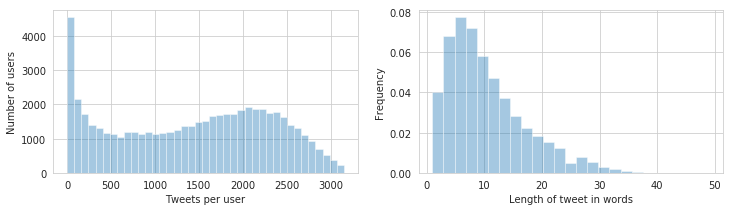
\includegraphics[width=\textwidth]{./images/dataset_histograms.png}
    \caption{Distributional figures of the dataset. Left: Distribution of number of tweets per user. Right: Distribution of length (in words) of tweets.} 
    \label{fig:tweets_distribution} 
 \end{figure*}

To gather our data, information of \textit{departments} in Argentina (the second-level administrative division of the country, after \textit{provinces}) was collected from the 2010 National Census.\footnote{\url{https://www.indec.gov.ar}} Next, a lookup was made through the Twitter API for users with location matching those departments, while balancing the number of users per province. The Python library \textit{tweepy} was used to interact with the Twitter API. 

Although we tried to retrieve users from every single department, we found that they concentrate mainly around larger cities. This phenomenon is due to limitations in the geographical information made available by Twitter. This is why we selected provinces as our geographical unit of study, rather than more fine-grained departments. We collected roughly 2400 users per province.

For these users, we retrieved their entire tweetlines. Tweets were tokenized using \emph{NLTK} \cite{bird2009natural}. Hashtags and mentions to users were removed; the remaining words were downcased; and identical consecutive vowels were normalized up to three repetitions (``woaaa'' instead of ``woaaaaaa''). Analogously to users, the number of words per province was also balanced. Table \ref{tab:summary_tweets} lists the figures for the collected dataset, and Figure \ref{fig:tweets_distribution} display the distributions of tweets per user and length of tweets.

\begin{table}[b]
\begin{center}

\begin{tabular}{lrrr}
            & Total   & Mean   & SD \\ % &           STD 
\hline 
Words       &  647M   &  28.14M & 6.64M  \\ %&  3.325680e+06 \\
Tweets      &  80.9M  &  3.51M  & 0.91M  \\ %&  4.571673e+05 \\
Users       &  56.2K  &  2.44K  & 0.04K  \\ %&  1.947665e+01 \\
Vocabulary  &   7.5M  &  0.32M  & 0.04M  \\ %&  2.619165e+04 \\
\hline
\end{tabular}


\caption{Dataset summary. Total figures are provided, along with province-level mean and standard deviation.}
\label{tab:summary_tweets}
\end{center}
\end{table}


It is well known that Twitter vocabulary tends to be very noisy \cite{kaufmann2010syntactic} with lots of contractions, non-normal spellings (e.g., vocalizations), typos, etc. Consequently, only words occurring more than 40 times and used by more than 25 users were taken into account. This removes about 1\% of the total words and reduces vocabulary from 2.3 million words to around 135 thousand words. 

While these preprocessing steps may seem insufficient for many linguistic analyses, we find them acceptable enough for our present study, given that the phenomenon of locally-used words will still be likely to emerge in spite of different spellings, typos and other morphological variations. Indeed, while the same word might appear with several variations or spellings, we expect at least one normalized form to be more frequent and thus stand out from the rest.









\subsection*{Metrics}


\begin{figure*}[t]
\centering
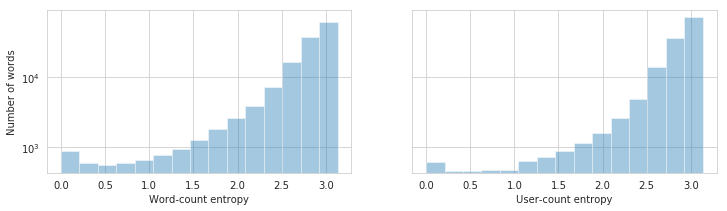
\includegraphics[width=\textwidth]{./images/entropies.png}
\caption{Histogram of word occurrence entropy ($H_w$). As one would expect, most words are used uniformly across the country} 
\label{fig:word_ocurrence_entropy} 
\end{figure*}


We can think of a \emph{regionalism} as a word whose use is not uniform across all the studied region, whose concentration is high in a specific part of the country. We are trying, in fact, to measure disorder of the use of a word, and there exists an information-theoretic tool for this: entropy.

It is known that entropy holds information about the semantic role played by a word \cite{montemurro2002entropic, montemurro2010towards}. High-entropy words, given a text, are more likely to be pronouns, connectors and other non-informative words, whereas its low-entropy counterparts are usually nouns and adjectives playing a key role in the document. 

Taking into account occurrence of words across a geographical region, words with high entropy (high disorder) can be regarded as words whose use is similar all across the region of study. On the other hand, low-entropy words are more used in a region than in the rest of it.

Let $p = (p_1, p_2, \ldots, p_N)$ the relative frequencies of occurrence of the word $\omega$ for each geographical region (in our case, provinces), the \emph{word-count entropy} is defined as:

\begin{equation}
    H_w(\omega) = -\sum \limits_{k=1}^{N} p_k \log(p_k)
\end{equation}


This measure does not take in account the frequency of words, which is also important. For instance, a word occurring once in a province has the same entropy as a word occurring millions of times at the same place. To remediate this issue, a measure based on \cite{montemurro2010towards} was developed, taking into account the frequency of use. We define the \emph{Information Value} of $w$ as:

\begin{equation}
  \label{eqn:iv_words}
  I_w(\omega) = p(\omega) \,  (\log(n) - H_w(\omega))
\end{equation}

The $log(n)$ in the formula represents the maximum possible value of $H(\omega)$ \cite{shannon2001mathematical}; for our work, recall that $n = 23$ (number of provinces in Argentina).

Another factor of information of a word is the amount of people using it on Twitter, something already used in previous works\cite{Cui:2012:DBE:2396761.2398519}. Using the same arguments as above, if $\omega$ is a word, and if $q_1, q_2, \ldots , q_n$ are the relative probabilities of a user of $\omega$ belonging to each province, we define the \emph{user-count entropy} as.

\begin{equation}
    H_p(\omega) = -\sum \limits_{k=1}^{N} q_k \log(q_k)
\end{equation}


Then, we define \emph{User-Count Information Value} of  $\omega$ as:

\begin{equation}
  \label{eqn:iv_users}
  I_p(\omega) = p(\omega) \, (\log(n) - H_p(\omega))
\end{equation}

This measures the concentration of the people using this word.  In \ref{fig:word_ocurrence_entropy} we can observe the distribution of \emph{Word-Count Entropy} and \emph{User-Count Entropy} for the words in our vocabulary. As one would expect, most words are used uniformly across the country —both in occurrences and in users of it.

To take into account both \emph{word-counts} and \emph{user-counts} we define a third measure called \emph{Mixed Information Value} as:

\begin{equation}
  I(\omega) = I_w(\omega)  I_p(\omega)
\end{equation}


High values of $I(w)$ are reached when information value on users and on ocurrences is also high.



Due to the Zipfian nature of the distribution of words, the frequency of use of the most-used words is many orders of magnitude higher than others. This phenomenon also occurs with the user count. So the $p(w)$ term in equations \eqref{eqn:iv_words} and \eqref{eqn:iv_users} becomes a problem as very frequent words would overcome their low entropy. To alleviate this, we performed a normalization on the word frequency as follows: let 

\begin{equation}
    M_w = \argmax\limits_{\omega \in W} \#\omega 
\end{equation}

we define then

\begin{equation}
    n_w(\omega) = \frac{\log(\# w)}{\log(M_w)}
\end{equation}

Due to the logarithm in the formula, terms with a high amount of occurrences have little difference of $n_w(\omega)$ between them.

In an analogous form, we define a normalization for the amount of people using a word, named $n_p$. Hence, we redefine our information measures as:

\begin{align}
  I_w(\omega) &= n_w(\omega) (\log(n) - H_w(\omega)) \\
  I_p(\omega) &= n_p(\omega) (\log(n) - H_p(\omega)) 
\end{align}




\subsection*{Lexicographic Validation}

\label{palabras_candidatas}





Based on the list of words identified as having a contrastive use in a region, we performed a linguistic validation of the first thousand words given by each metric. It consisted of a detailed study, word by word, to determine if the word in question is part of the lexical repertoire of a community of speakers. 

This excluded, as is traditional in lexicography, proper and local place names. These words occur mostly in their respective regions, having high entropy and also a high number of occurrences, hence resulting in high values for our metrics. To facilitate the detection of regionalisms, we automatically highlighted words suspected to be toponyms so that the team of lexicographers have a first warning about it.

A team of lexicographers analyzed the first thousand words for each metric. Along these lists, they were provided with tables having figures for each word and province: users, occurrences and normalized frequency (ocurrences per million words). Table \ref{tab:metric_results} shows the results of this labeling. Using information of the number of users of a word seems to be capturing the highest number of words marked as regionalisms. 

\todo{Agregamos algo sobre que "exploramos más palabras" que las primeras 1000? o lo dejamos ahí?}
From these words marked as regionalisms, lexicographers performed a characterization of the results according to the linguistic phenomenon they represent. Table \ref{tab:characterisation} displays lexicographic groups among the regionalisms found in the analyzed words with examples. Table \ref{tab:guaranitic} displays occurrences of three outstanding examples: words coming from guaranitic region.

\todo{Que agregue algo más Santiago sobre esto}. 



\todo{Chequear estos números!!!!}
\begin{table}[hb]
    \centering
    \begin{tabular}{l c c}
    Word & Guaranitic Region & Litoral Region \\
    \hline
    angá & 32.80 & 0.33 \\
    angaú & 8.42 & 0.03 \\
    mitaí & 15.06 & 0.04 \\
    \hline
    \end{tabular}
    \caption{Guaranitic words and its occurrences per million in two different dialectal regions}
    \label{tab:guaranitic}
\end{table}




\begin{table*}[ht!]
\centering

\begin{tabular}{p{0.15\textwidth} p{0.1\textwidth} p{0.65\textwidth}}

Group               & Province & Example  \\ % &           STD \\

\hline
Colloquialisms      & Córdoba & \blockquote{Perdon pero tenes que ser muy \textbf{culiado} para ir a mc y pedirte una ensalada}   \\
& Mendoza & \blockquote{Q \textbf{chombi} hacer un chiste y q la otra persona no se ría o no lo entienda} \\
& Formosa & \blockquote{Tenía la re expectativa para este sábado y al final \textbf{trancó} todo} \\


\hline
Colloquialisms with a verbal or noun base& Buenos Aires &   \blockquote{Me vine a acostar y ya me dicen que parezco de 80 años ME CHUPA UN HUEVO LO QUE PIENSEN, DEJENME \textbf{ABUELEAR} } \\

& Neuquén & \blockquote{Me calma mucho \textbf{mimosear} a mi perro } \\

& Tierra del Fuego & \blockquote{Estaría bueno que ari venga aunque sea a saludarme y que no se quede todo el tiempo \textbf{pollereando}.} \\


\hline \\

Indigenisms        &  Formosa & \blockquote{Te regalo ser \textbf{mitaí} y ir a jurar la bandera con el guardapolvo caliente ese y la corbata que te ahorca todo} \\
& Corrientes & \textbf{Angá} mi negrito, esta triste \\
& Tucumán & Gracias tormenta \textbf{ura} por sonar como una pochoclera de chasquibums a las 3 de la mañana en mi ventana \\
\hline

Words alluding regional reality & San Juan & \blockquote{Quiero a alguien que me diga vamos a comer \textbf{piadinas}, un pancho, un chori, una hamburguesa lo que sea y soy feliz} \\

& Misiones & \blockquote{\textbf{Tareferos} que reclamaban asistencia interzafra en Posadas estarían preparando una protesta para hoy en la Fiesta del Inmigrante en Oberá.} \\
& Jujuy & \blockquote{Me encantan los bohemios anti sistema que usan vans. Es como que seas ecologista y uses un cuaderno hecho con media \textbf{yunga}.} \\


\hline

``Leism'' & Misiones &  \blockquote{No te olvides de \textbf{saludarle} a tu suegro hoy} \\

& Misiones &   \blockquote{Vine a \textbf{visitarle} a mis primas y estan re colgadas, para eso me quedaba en mi casa no maaa } \\

& Formosa & \blockquote{A \textbf{esperarle} a nahuel, que traiga los teresss } \\

\hline
Fusions and acronyms & Buenos Aires & \blockquote{Los sueños de la siesta me dejan \textbf{patra} }\\

%   \blockquote[Córdoba]{Si mañana me dice q no, voy sola, necesito ver esa pelicula en el cine siosi}

\hline

Words with different meaning in a region & Mendoza &  \blockquote{Mañana que alguien \textbf{atine} con parque y porrones} \\

& San Juan & \blockquote{\textbf{Mansas} ganas de sentarme a tomar un te con semitas} \\

& Tierra del Fuego &  \blockquote{\textbf{Habilítenme} una nueva espaldaa} \\

& San Juan &  \blockquote{sigo \textbf{asada} por cosas que han pasado hace como dos dias, que falla (Mendoza) / Que \textbf{asada} estoy, tengo la cabeza echa un lío} \\


\hline

Intejerctions & Formosa &   \blockquote{\textbf{Aijué}, encima me decís vieja, re que no pinta esto facundo jaja ya te dije como es la onda, fin } \\

& Formosa &  \blockquote{\textbf{Ains}, una mujer hablando de fútbol.} \\

& Corrientes & \blockquote{Al fin una buena: hora libreeee! \textbf{Yirr} } \\
 

\hline 
\end{tabular}
\caption{Characterisation of the regionalisms found in the analysis.  }

\label{tab:characterisation}
\end{table*}




\section{Results}


\begin{figure*}[t]
   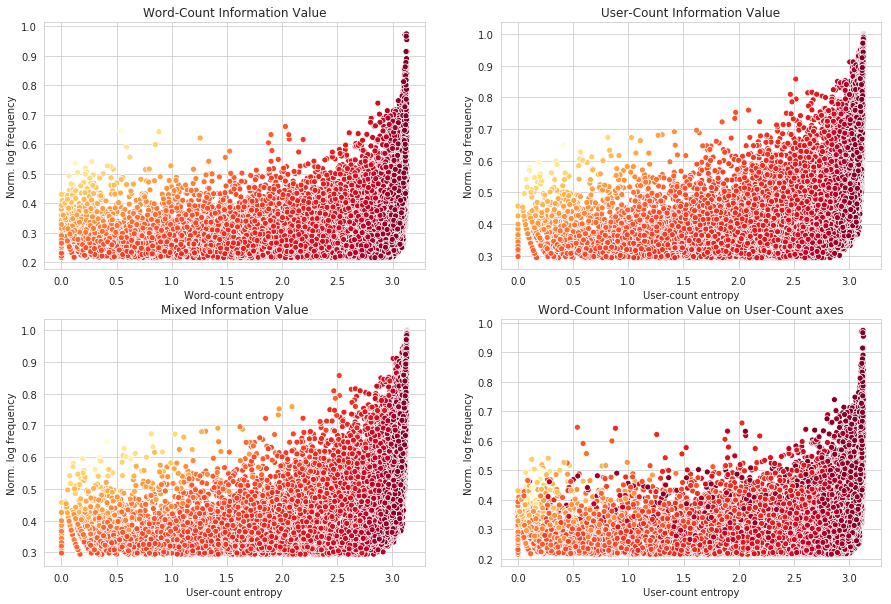
\includegraphics[width=\textwidth]{./images/entropy_log_rank.png}
   \label{fig:ivalue}
   \caption{Scatter plot of words. Horizontal axis represents user-count entropy, vertical axis represents the normalized log user-frequency of the word, and colour indicates User-count Information Value: lighter means higher value}
\end{figure*}



Figure \ref{fig:ivalue} displays the log-frequency and Entropy of words, along with the value of the respective metric. As we can see (both in the User-Count and Word-Count plots) the words we rank high in our lists are those closer to the upper-left of the plot — that is, highly-concentrated and occurring a consideriable number of times. Mixed Information Value seems to respect the User-Count order, and the last plot shows that although User-Count and Word-Count ranks are similar, they are not exactly the same as shown by the ``darker'' points close to the upper-left corner.

\todo{Agregar un listado de las 10 primeras palabras de cada listado?}

Regarding the lexicographic validation, Table \ref{tab:metric_results} display the percentage of words marked as being lexicographically interesting. The number of users of a word alone seems to be the most informative feature. 

\begin{table}[t]
\centering
\begin{tabular}{lr}
Metric                      &  \% of interesting words  \\ % &           STD \\
\hline
Word-Count       &  21.9\%   \\
User-Count       &  30.2\%  \\
Mixed            &  25.3\%  \\ %&  1.947665e+01 \\
\hline
\end{tabular}
\caption{Results of the metrics. The percentage of detected regionalisms in the first 1000 words is given for each metric: Word Information Value, User Information Value, and Mixed Information Value  }
\label{tab:metric_results}
\end{table}




\section{Discussion}

Although there are no other projects that provide a comparison term to assess the degree of success involved in this relationship, there is no doubt that, at least in the detection of local colloquialisms \todo{cambiar a "regionalism"}currently in use, the tool poses a real point of inflection for contrastive lexicography. This area of the lexicon is just the most elusive, since its impact on any printed medium arrives noticeably later and, even more important, in most cases it never reaches. Several words that are already included in the Dictionary of the Speech of Argentines \cite {academia2008diccionario} were included as relevant, given that this fact is an additional confirmation of the relevance of the location that assigned the metric.


It is worth mentioning that words coming from \emph{guaraní} —language spoken in Northern Argentina, Paraguay, Bolivia and Southwest of Brazil— coincide with the region delimited by \cite{vidal1964espanol}. An example of this phenomenon are the words \textit{angá}, \textit{angaú} y \textit{mitaí}.

- Agregar que esto aplica no sólo a encontrar regionalismos sino temas/términos que sean propios de una región geográfica particular (marketing, ver penetración de una marca como en una de las citas).
\section{Conclusions}
In this multidisciplinary work, we developed and compared three novel metrics to detect regionalisms on Twitter based on Information Theory. One of these metric was based on the occurrences of a word (\wordmetric), another based on the number of users of a word (\usermetric), and the third combined the other two (\mixedmetric). A team of lexicographers annotated the first thousand words as ranked by each of these metrics to assess the presence of regionalisms, and \usermetric{} yielded the best results, suggesting that the number of users of a word is more informative than its usage frequency.

This method aided lexicographers in their task, letting them
%add a number of words into the 2019 version of 
propose the addition of a number of words into 
%%anonimizacion, cambiar en la version final
the \emph{Diccionario del Habla de los Argentinos}. In the case of this particular dictionary, work relies on a collaborative effort that is based on the intuition of academics and lexicographers that identify regionalisms used mainly (seldom exclusively) within Argentina's borders by carefully parsing over a diversity of sources. This method, albeit effective, can hardly aspire to be comprehensive. Therefore, the promise shown by the present approach does not limit itself to avoiding most of this manual work, which, in and of itself, would already be a sizeable contribution. Since a considerable portion of the lexical repertoire of a community does not make its way across to published materials (which make most of the 300 millions words included to date in, for example, CORPES XXI \cite{espanolabanco}), the possibility of creating lists of words that are likely to be regional, based on actual written utterances by users, opens a way of shedding light onto entire pockets of lexical items that would remain otherwise chronically underrepresented in dictionaries. Even when a regional word is published, and then included in corpora, the task of appropriately isolating it remains largely unchanged, given that the word has to previously be identified in order to then take advantage of the statistical information available. Should the opportunity present itself, the potential for using Information Theory in this way with corpora like CORPES XXI is very significant.

Finally, a challenge triggered by this work is the detection of regions with different dialectal uses as done in previous works \cite{gonccalves2014crowdsourcing}, but using features obtained in a semisupervised fashion with our metrics. This would allow to assess the validity of the dialectal regions of Argentina proposed by Vidal de Battini in 1964 \cite{vidal1964espanol}. Also, spatial and temporal information could be explored to further enhance the precision of this method. 





\section{Contributors to this document}
\label{sec:contributors}

This document was adapted by Lillian Lee and Kristina Toutanova
from the instructions and files for ACL 2018, by Shay Cohen, Kevin Gimpel, and
Wei Lu. Those files were drawn from earlier *ACL proceedings, including those
for ACL 2017 by Dan Gildea and Min-Yen Kan, NAACL 2017 by Margaret Mitchell,
ACL 2012 by Maggie Li and Michael White, those from ACL 2010 by Jing-Shing
Chang and Philipp Koehn, those for ACL 2008 by Johanna D. Moore, Simone
Teufel, James Allan, and Sadaoki Furui, those for ACL 2005 by Hwee Tou Ng and
Kemal Oflazer, those for ACL 2002 by Eugene Charniak and Dekang Lin, and
earlier ACL and EACL formats,  which were written by several people,
including John Chen, Henry S. Thompson and Donald Walker. Additional elements
were taken from the formatting instructions of the {\em International Joint
Conference on Artificial   Intelligence} and the \emph{Conference on Computer
Vision and Pattern Recognition}.


\bibliography{tacl2018}
\bibliographystyle{acl_natbib}

\end{document}


